\documentclass[11pt,a4paper]{article}
\usepackage[margin=1in]{geometry}
\usepackage[T1]{fontenc}
\usepackage[utf8]{inputenc}
\usepackage{lmodern}
\usepackage{microtype}
\usepackage{amsmath,amssymb}
\usepackage{graphicx}
\usepackage{xcolor}
\usepackage[hidelinks]{hyperref}

\definecolor{accent}{HTML}{0F766E}
\definecolor{rulegray}{HTML}{D1D5DB}

\setlength{\parindent}{0pt}
\setlength{\parskip}{0.55em}

\begin{document}

{\color{accent}\rule{\linewidth}{1.2pt}}

\vspace{0.6em}
{\LARGE\bfseries Stability Time from an Underdamped Second-Order Model\par}
{\large From \texttt{gnn.png} and \texttt{dM\_dt.png} to a practical value of $t_{stable}$\par}

\vspace{0.35em}
{\color{accent}\rule{\linewidth}{0.8pt}}

\[
t_s \approx 2\,\mathrm{s},
\qquad
\tau \approx 2\,\mathrm{s},
\qquad
t_{stable} \approx 10\,\mathrm{s}.
\]

\section*{1. From \texttt{gnn.png} to the model}
The curve in \texttt{gnn.png} has four features:
\[
\text{rise} \;\to\; \text{overshoot} \;\to\; \text{decaying oscillation} \;\to\; \text{final value}.
\]
This is the standard signature of an \textbf{linear underdamped second-order system}.  
\begin{figure}[htbp]
  \centering
  \setlength{\fboxsep}{0pt}
  \fcolorbox{rulegray}{white}{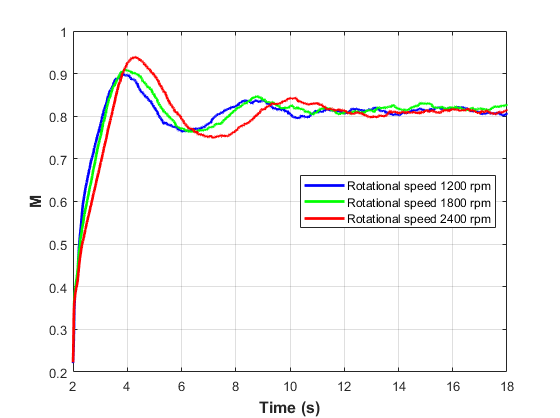
\includegraphics[width=0.72\linewidth]{gnn.png}}
  \caption{Observed response used to motivate the underdamped second-order model.}
\end{figure}

We model it by
\[
\ddot M + 2\zeta\omega_n \dot M + \omega_n^2(M-M_{\infty}) = 0,
\qquad t \ge t_s.
\]

Let
\[
u=t-t_s,
\qquad
\tau = \frac{1}{\zeta\omega_n},
\qquad
\omega_d=\omega_n\sqrt{1-\zeta^2}.
\]
Then the underdamped response has the form
\[
M(t)=M_{\infty}+e^{-u/\tau}\left(A\cos(\omega_d u)+B\sin(\omega_d u)\right).
\]

For the step-like case with
\[
M(t_s)=M_0,
\qquad
\dot M(t_s)=0,
\qquad
\Delta M=M_{\infty}-M_0,
\]
we obtain
\[
M(t)=M_{\infty}
-\Delta M\,e^{-u/\tau}
\left[
\cos(\omega_d u)
+\frac{\zeta}{\sqrt{1-\zeta^2}}\sin(\omega_d u)
\right].
\]

\section*{2. Stability Time from the model}
The transient error is
\[
e(t)=M(t)-M_{\infty}.
\]
Its envelope decays as
\[
|e(t)| \propto e^{-u/\tau}.
\]
Also,
\[
\left|\frac{dM}{dt}\right| \propto e^{-u/\tau}.
\]

Therefore a compact practical rule is
\[
t_{stable}\approx t_s+4\tau.
\]
Useful variants:
\[
t_s+3\tau \;\text{: loose},
\qquad
t_s+4\tau \;\text{: recommended},
\qquad
t_s+5\tau \;\text{: conservative}.
\]

\section*{3. Estimate $\tau$ from the two plots}
\begin{figure}[htbp]
  \centering
  \begin{minipage}[t]{0.475\linewidth}
    \centering
    \setlength{\fboxsep}{0pt}
    \fcolorbox{rulegray}{white}{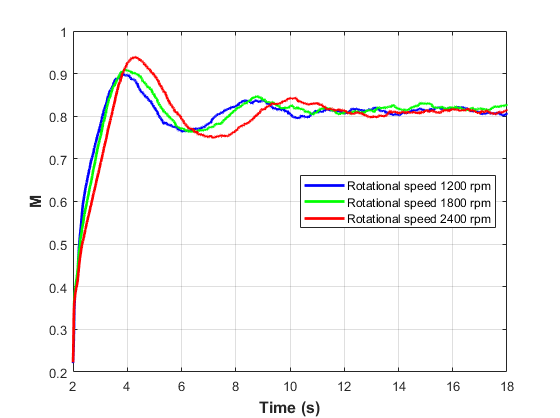
\includegraphics[width=0.985\linewidth]{gnn.png}}
  \end{minipage}
  \hfill
  \begin{minipage}[t]{0.475\linewidth}
    \centering
    \setlength{\fboxsep}{0pt}
    \fcolorbox{rulegray}{white}{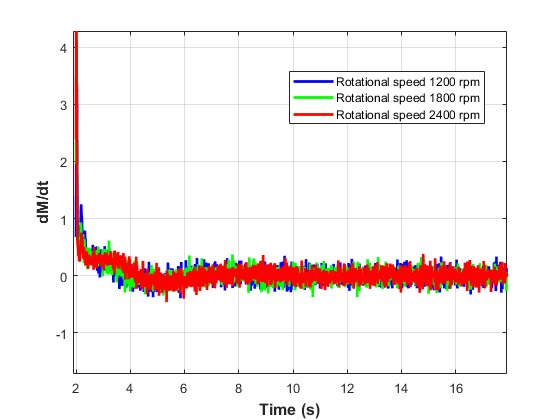
\includegraphics[width=0.985\linewidth]{dM_dt.png}}
  \end{minipage}
  \caption{Left: $M(t)$. Right: $dM/dt$.}
\end{figure}

From \texttt{gnn.png}, the transient starts at about
\[
t_s \approx 2\,\mathrm{s}.
\]

From \texttt{dM\_dt.png}, the derivative envelope drops from order
\[
|\dot M| \sim 4
\quad \text{near } t\approx 2\,\mathrm{s}
\]
to order
\[
|\dot M| \sim 0.08
\quad \text{near } t\approx 10\,\mathrm{s}.
\]
Hence
\[
\frac{0.08}{4}\approx 0.02 \approx e^{-4}.
\]
Using the decay law
\[
|\dot M(t)| \propto e^{-(t-t_s)/\tau},
\]
we get
\[
e^{-(10-2)/\tau}\approx e^{-4}
\quad \Rightarrow \quad
\tau \approx 2\,\mathrm{s}.
\]

\section*{4. Numerical value of $t_{stable}$}
Substitute the estimated $\tau$ into the recommended rule:
\[
t_{stable}\approx t_s+4\tau
\approx 2 + 4\times 2
= 10\,\mathrm{s}.
\]

If a safer margin is needed:
\[
t_{stable}\approx t_s+5\tau
\approx 2 + 5\times 2
= 12\,\mathrm{s}.
\]

\[
\boxed{t_{stable}\approx 10\,\mathrm{s}}
\qquad
\boxed{t_{stable}\approx 12\,\mathrm{s}\ \text{(conservative)}}.
\]

\end{document}
